\documentclass{cubeamer}

\usepackage{trimclip}
\usepackage{wrapfig}
\usepackage{graphicx}
\usepackage{caption}
\usepackage{subcaption}
\usepackage{multicol}
\usepackage{tikz}

\usetikzlibrary{positioning}
\usetikzlibrary{arrows.meta}
\usetikzlibrary{arrows,shapes,backgrounds}
\usepackage{amsmath,amsfonts}

\newcommand{\btVFill}{\vskip0pt plus 1filll}


\title{Embedding Intuitionistic into Classical Logic}
\subtitle{LPAR-24}
\author[A. Pluska, F. Zuleger]{Alexander Pluska, Florian Zuleger}
\date{\today} % or whatever the date you are presenting in is
\institute[TU Vienna]{Vienna University of Technology}
% \copyrightnotice{Published by the American Institute of Aeronautics and Astronautics, Inc., with permission}

\begin{document}
	
	\maketitle
	
	\cutoc
	
	\section{Background}
	
	\begin{frame}{Languages}
		Propositional Logic:
		\begin{itemize}
			\item Propositional variables $A, B, C, \dots$ and bottom $\bot$.
			\item Connectives $\wedge, \vee, \to$.
		\end{itemize}
		\[((A\to\bot)\vee B)\wedge C\]
		First-order Logic:
		\begin{itemize}
			\item Ambient Signature $\Sigma$.
			\item Inductively defined terms from variables and function symbols.
			\item Atoms from predicate symbols, equalities between terms and $\bot$.
			\item Connectives $\wedge, \vee, \to$ and quantifiers $\forall, \exists$.
		\end{itemize}
		\[\forall x (P(x)\to (f(x) = c\wedge \exists y Q(f(x), g(y))))\]
	\end{frame}
	
	
	\begin{frame}{Intuitionistic Logic}
		\begin{figure}[!tbp]
			\centering
			\begin{subfigure}[][][t]{0.6\textwidth}
				\begin{itemize}
					\item Motivation:
					\begin{itemize}
						\item Mathematical Constructivism.
						\item Curry-Howard-Correspondence.
					\end{itemize}
					\item Not intuitionistically valid:
					$$A\vee\neg A\hspace*{1cm} \forall x\neg\neg A(x)\to \neg\neg\forall x A(x)$$
					\item Classical Logic $\longrightarrow$ Intuitionisic logic:\[ \text{Double Negation Translation}\]
					\item Intuitionistic Logic $\longrightarrow$ Classical Logic\[\text ?\]
				\end{itemize}
			\end{subfigure}
			\hfill
			\begin{subfigure}[]{0.3\textwidth}
				\centering
				\includegraphics[width=0.9\textwidth]{logicians.png}
				\caption{L. E. J. Brouwer, A. Heyting, H. B. Curry, W. A. Howard}
			\end{subfigure}
		\end{figure}
	\end{frame}
		

	\begin{frame}{Existing approaches}
		\begin{figure}
			\begin{subfigure}{0.49\textwidth}
				\centering
				\includegraphics[width=\textwidth]{friedman.png}
			\end{subfigure}
			\begin{subfigure}{0.49\textwidth}
				\centering
				\includegraphics[width=\textwidth]{schwichtenberg.png}
			\end{subfigure}
		\vspace{.5cm}
			\begin{subfigure}[b]{0.49\textwidth}
				\centering
				\includegraphics[width=\textwidth]{griffin.png}
			\end{subfigure}
			\begin{subfigure}[b]{0.49\textwidth}
				\centering
				\includegraphics[width=0.9\textwidth]{parigot.png}
			\end{subfigure}
		\end{figure}
	\end{frame}

	\begin{frame}{Kripke Semantics}
		\centering
		\vspace*{1cm}
		\begin{tabular}{c|c}
			Classical Logic&Intuitionistic Logic\\
			\hline
			Single valuation $v$.&Partially ordered set $W$ of worlds and family of\\&valuations $(v_u)_{u\in W}$ satisfying \emph{persistency}.\\
			\hline
			$v\models\varphi$&$u\models\varphi$ for each $u\in W$.	
		\end{tabular}
		\vspace*{.5cm}

		For atoms: $u\models A$ iff $v_u\models A$.\\
		Inductive extensions to formulas generally as in the first order case, e.g. \[u\models \varphi\wedge\psi \text{ iff } u\models\varphi \text{ and } u\models\psi.\]\vspace*{1.5cm}
		Difference: $u\models\varphi\to\psi$ iff \textbf{for all} $\mathbf{w}\geq \mathbf{u}$ we have $w\models\varphi$ or $w\models\psi$.
	\end{frame}
	
	
	\begin{frame}{Kripke Semantics - Example}
		\begin{figure}[!tbp]
		\centering
		\begin{subfigure}[][][t]{0.3\textwidth}
			\centering
				$A\vee\neg A\:\approx$ ``$A$ or never $A$''\vspace*{1cm}
				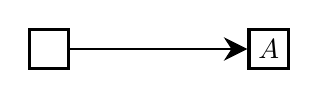
\begin{tikzpicture}[squarednode/.style={rectangle, draw, very thick, minimum size=5mm}]
					\node (center) {};
					\node[squarednode]      (left)   [left=of center] {};
					\node[squarednode]      (right)       	[right=of center] {$A$};
					\draw[-{Stealth[length=3mm, width=3mm]}] (left.east) -- (right.west);	
				\end{tikzpicture}
			\caption{Counter-model $A\vee\neg A$ $A\vee(A\to\bot)$}
		\end{subfigure}
			\hfill
		\begin{subfigure}[][][t]{0.6\textwidth}
			\centering
			$\forall x\neg\neg A(x)\to \neg\neg\forall x A(x)\:\approx$ ``for all $x$ eventually $A(x)$ implies eventually for all $x$ $A(x)$''\vspace*{1cm}
			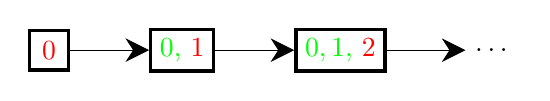
\begin{tikzpicture}[squarednode/.style={rectangle, draw, very thick, minimum size=5mm}]
				\node[squarednode]  (0) {\color{red}$0$};
				\node[squarednode]      (1)   [right=of 0] {\color{green}$0$, \color{red}$1$};
				\node[squarednode]      (2)       	[right=of 1] {\color{green}$0, 1$, \color{red}$2$};
				\node   (3)       	[right=of 2] {\dots};
				\draw[-{Stealth[length=3mm, width=3mm]}] (0.east) -- (1.west);	
				\draw[-{Stealth[length=3mm, width=3mm]}] (1.east) -- (2.west);
				\draw[-{Stealth[length=3mm, width=3mm]}] (2.east) -- (3.west);	
			\end{tikzpicture}
			\caption{Counter-model $\forall x\neg\neg A(x)\to \neg\neg\forall x A(x)$}
		\end{subfigure}
		\end{figure}
	\end{frame}

	\begin{frame}{A second motivation: Automated Deduction for Intuitionistic Logic}
		\begin{figure}
		\begin{subfigure}[b]{\textwidth}
			\centering
				\includegraphics[width=\textwidth]{iltp.png}
			\caption{ILTP benchmark}
		\end{subfigure}
		\begin{subfigure}[b]{\textwidth}
			\includegraphics[width=\textwidth]{CASC.png}
			\caption{CASC-28 Results}
		\end{subfigure}
		\end{figure}
	\end{frame}


	\begin{frame}{Not quite CNF}
		\begin{lemma}[Intuitionistic normal form, propositional case]
	For every propositional formula $\varphi$ there exists an atom $P$ as well as sets of clauses $\mathcal R, \mathcal X$, with $\mathcal R$ containing  \emph{flat clauses} of the form
	$$\bigwedge_iA_i\to\bigvee_jB_j$$
	and $\mathcal X$ containing \emph{implication clauses} of the form
	$(A\to B)\to C,$
	such that $\varphi$ is intuitionistically equivalid to
	$$\left(\bigwedge\mathcal R\wedge\bigwedge\mathcal X\right)\to P$$where $A_i, B_i, A, B, C$ are atomic.
			\end{lemma}	
	\end{frame}

	\begin{frame}{Not quite CNF - Example}
		The formulas \[A\vee\neg A\] and \[((A\to P)\wedge(\neg A\to P))\to P\] are intuitionistically equivalid.
	\end{frame}
	
	\begin{frame}{Not quite CNF - First-order case}
		In addition to sets of flat clauses $\mathcal R$ of the form
	$$\forall\vec x\left(\bigwedge A_i\to\bigvee B_j\right)$$ and implication clauses $\mathcal X$ of the form
	$$\forall\vec x((A\to B)\to C)$$ there is a set of \emph{quantification clauses} $\mathcal Q$ of the form $$\forall \vec x(\forall \vec yQ\to P).$$
	\end{frame}
	

	
	\section{The Embedding}
	
	\begin{frame}{Overview}
		\begin{enumerate}
			\item Encoding of Kripke Semantics
			\item Reduction of the Encoding
		\end{enumerate}
	\end{frame}

	\begin{frame}{Classical Encoding of Kripke Semantics - Propositional Case}
		\begin{lemma}
			Let $\varphi$ be a propositional formula.
		 	We can inductively define $\varphi^{b}$ 
			and have $K(\varphi)$ encode the theory of Kripke structures, i.e.
			\[K(\varphi) := \text{\normalfont PartialOrder}(\preceq)\wedge\forall u\forall w(u\preceq w\to \text{\normalfont Persistent}(u, w)),\]
			such that
			\[\varphi^{C} := K(\varphi)\to \varphi^{b}\]
		    is classically valid if and only if $\varphi$ is intuitionistically valid.
		\end{lemma}
		In this process propositional variables are replaced by unary predicates, where $M, [u/x]\models A(x)$ can be interpreted as $u\models A$.
	\end{frame}
	
	\begin{frame}{Reducing the Encoding - Propositional Case}
		\vspace*{.5cm}
		\begin{lemma}
			Let $\Lambda$ be the set of sequences without repetition over $\mathcal X$. A countermodel to $\varphi^C$ exists if and only if a countermodel with domain $\Lambda$ exists in which $\preceq$ is interpreted as the prefix ordering.
		\end{lemma}
		\btVFill
		Recall: Intuitionistic normal from $\left(\bigwedge\mathcal R\wedge\bigwedge\mathcal X\right)\to P$ with $\mathcal R$ containing  \emph{flat clauses} $\bigwedge A_i\to \bigvee B_j$ and $\mathcal X$ containing \emph{implication clauses} $(A\to B)\to C$.
	\end{frame}

	
	\begin{frame}{Reducing the Encoding - Propositional Case}
		\vspace*{.5cm}
		\begin{lemma}
			Let $\Lambda$ be the set of sequences without repetition over $\mathcal X$. A countermodel to $\varphi^C$ exists if and only if a countermodel exists with domain $\Lambda$ exists and in which $\preceq$ is interpreted as the prefix ordering.
		\end{lemma}
		Example, $((A\to P)\wedge(\neg A\to P))\to P$:
		\begin{center}
		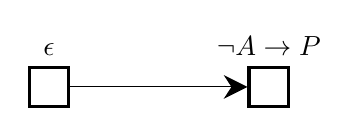
\begin{tikzpicture}[squarednode/.style={rectangle, draw, very thick, minimum size=5mm}]
			\node (center) {};
			\node[squarednode]      (left)   [left=of center, label=$\epsilon$] {};
			\node[squarednode]      (right)       	[right=of center, label=$\neg A\to P$] {};
			\draw[-{Stealth[length=3mm, width=3mm]}] (left.east) -- (right.west);	
		\end{tikzpicture}
		\end{center}
		\btVFill
		Recall: Intuitionistic normal from $\left(\bigwedge\mathcal R\wedge\bigwedge\mathcal X\right)\to P$ with $\mathcal R$ containing  \emph{flat clauses} $\bigwedge A_i\to \bigvee B_j$ and $\mathcal X$ containing \emph{implication clauses} $(A\to B)\to C$.
	\end{frame}

	\begin{frame}{Reducing the Encoding - Propositional Case}
		\vspace*{.5cm}
		\begin{lemma}
			Let $\Lambda$ be the set of sequences without repetition over $\mathcal X$. A countermodel to $\varphi^C$ exists if and only if a countermodel exists with domain $\Lambda$ exists and in which $\preceq$ is interpreted as the prefix ordering.
		\end{lemma}
		Example, $((A\to P)\wedge(\neg A\to P))\to P$:
		\begin{center}
		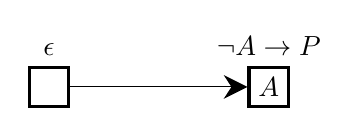
\begin{tikzpicture}[squarednode/.style={rectangle, draw, very thick, minimum size=5mm}]
			\node (center) {};
			\node[squarednode]      (left)   [left=of center, label=$\epsilon$] {};
			\node[squarednode]      (right)       	[right=of center, label=$\neg A\to P$] {$A$};
			\draw[-{Stealth[length=3mm, width=3mm]}] (left.east) -- (right.west);	
		\end{tikzpicture}
		\end{center}
		\btVFill
		Recall: Intuitionistic normal from $\left(\bigwedge\mathcal R\wedge\bigwedge\mathcal X\right)\to P$ with $\mathcal R$ containing  \emph{flat clauses} $\bigwedge A_i\to \bigvee B_j$ and $\mathcal X$ containing \emph{implication clauses} $(A\to B)\to C$.
	\end{frame}


	\begin{frame}{Reducing the Encoding - Propositional Case}
		\vspace*{.5cm}
		\begin{lemma}
			Let $\Lambda$ be the set of sequences without repetition over $\mathcal X$. A countermodel to $\varphi^C$ exists if and only if a countermodel exists with domain $\Lambda$ exists and in which $\preceq$ is interpreted as the prefix ordering.
		\end{lemma}
		\begin{corollary}[Small Model Property]
			If $\varphi$ is intuitionistically invalid then there exists a Kripke counter-model which is a rooted tree with height and degree bounded by $|\mathcal X|$.
		\end{corollary}
		\btVFill
		Recall: Intuitionistic normal from $\left(\bigwedge\mathcal R\wedge\bigwedge\mathcal X\right)\to P$ with $\mathcal R$ containing  \emph{flat clauses} $\bigwedge A_i\to \bigvee B_j$ and $\mathcal X$ containing \emph{implication clauses} $(A\to B)\to C$.
	\end{frame}
	

	
	\begin{frame}{Propositional Encoding}
		Knowing the shape of potential countermodels we can essentially replace universal quantification by enumeration. This gives us an embedding into propositional logic.
		\begin{itemize}
			\item For each atom $A$ and $\lambda\in\Lambda$ consider a new atom $A^\lambda$.
			\item $\bigwedge A_i\to \bigvee B_j$ is encoded as $\bigwedge \{\bigwedge A_i^\lambda\to \bigvee B_j^\lambda\mid \lambda\in\Lambda\}$.
			\item $\psi = (A\to B)\to C$ is encoded as $\bigwedge\{(A^{\lambda\psi}\to B^{\lambda\psi})\to C^\lambda\mid \lambda\in\Lambda, \psi\notin\lambda\}$.
			\item $P$ is encoded as $P^\epsilon$.
		\end{itemize}
		Size of the new formula is in $\mathcal O(|\varphi|\cdot 2^{|\mathcal X|})$.
		\btVFill
		Recall: Intuitionistic normal from $\left(\bigwedge\mathcal R\wedge\bigwedge\mathcal X\right)\to P$ with $\mathcal R$ containing  \emph{flat clauses} $\bigwedge A_i\to \bigvee B_j$ and $\mathcal X$ containing \emph{implication clauses} $(A\to B)\to C$.
	\end{frame}
	
	\begin{frame}{Aside - Encoding to QBF}
		\vspace*{2cm}
				
		\begin{lemma}
			For each propositional formula $\varphi$ there is effectively a QBF $\varphi^Q$ with $\mathcal |\varphi^Q|\in\mathcal O(|\mathcal R|\cdot|\mathcal X| + |\mathcal X|^3)$ such that $\varphi$ is intuitionistically invalid if and only if $\varphi^Q$ is a satisfiable QBF.
		\end{lemma}
		\btVFill
		Recall: Intuitionistic normal from $\left(\bigwedge\mathcal R\wedge\bigwedge\mathcal X\right)\to P$ with $\mathcal R$ containing  \emph{flat clauses} $\bigwedge A_i\to \bigvee B_j$ and $\mathcal X$ containing \emph{implication clauses} $(A\to B)\to C$.
	\end{frame}

	\begin{frame}{Classical Encoding of Kripke Semantics - First-order Case}
		\begin{itemize}
			\item Classical models must contain elements both representing worlds in the Kripke frame and elements in the domain of the models at each world.
			\item 
			We use a special predicate $E$ to encode that an element exists at a world.
		\end{itemize}
		As in the propositional case we can define $\varphi^b$ and encode the Kripke Semantics
		\begin{align*}
			K(\varphi)= &\:\text{PartialOrder}(\preceq) \to \forall u \forall w (u\preceq w\to \text{DomainSubset}(u, w))\\
			&\to\forall u(\text{DomainClosed}(u))\to \forall u\forall w (u\preceq w\to \text{Persistent}(u, w))
		\end{align*}
		such that
		\[\varphi^C:= K(\varphi)\to E(sk_0, b)\to \vec E(\vec a, b)\to \varphi^b\]
		is classically valid if and only if $\varphi$ is intuitionistically valid.
	\end{frame}
	
	\begin{frame}{Reducing the Encoding - First-order Case}
		\begin{itemize}
			\item We show that most model reduction techniques from the propositional case carry over to the first-order case.
			\item We are able to completely eliminate $\preceq$.
			\item It is \textbf{not} possible to completely eliminate quantification over worlds as some sentences only have counter-models with an infinite number of worlds.
			\item Redundant clauses can encode further model reductions.
			\item No exponential blowup \textbf{but} new symbols.
		\end{itemize}
	\end{frame}

	\section{Benchmark}
	
	\begin{frame}{Banchmark}
		\begin{itemize}
			\item Translation written in Rust.
			\item Classical backend: Vampire.
			\item ILTP library, 2670 problems.
			\item Problem \textsc{SYN007+1} removed.
			\item Intuitionistic SOTA provers for comparison:
			\begin{itemize}
				\item ileanCoP 1.2
				\item nanoCoP-i 2.0
			\end{itemize}
		\end{itemize}
	\end{frame}

	\begin{frame}{Benchmark}
		\begin{figure}
			\begin{subfigure}{0.39\textwidth}			
				\centering
					\begin{tabular}{l|c|c}
						Embedding&571&21.4\%\\
						Emb. (idem.)&557&20.9\%\\
						ileanCoP 1.2&875&32.8\%\\
						nanoCoP-i 2.0&858&32.1\%\\\hline
						Total&2669&100\%
					\end{tabular}
					\vspace{1.2cm}
					\caption{Solved problems by each prover.}
			\end{subfigure}	
			\begin{subfigure}{0.6\textwidth}
				\centering
				\includegraphics[width=0.66\textwidth]{circleplot.png}
				\caption{Instances proven by combinations of Embedding (red), Embedding (idem.) (green), ileanCoP or nanoCoP (blue)}
			\end{subfigure}
		\end{figure}
	\end{frame}
	
	\begin{frame}{Benchmark}
		\begin{figure}
			\begin{subfigure}{\textwidth}			
				\centering
					\begin{tabular}{c|c|lr|lr|lr|lr|c}
		$|\mathcal Q|$&$|\mathcal X|$&\multicolumn{2}{c}{Embedding}&\multicolumn{2}{c}{Emb. (idem.)}&\multicolumn{2}{c}{ileanCoP}&\multicolumn{2}{c}{nanoCoP-i 2.0}&Total\\\hline
		0&0		&157&88.2\%	&157&88.2\%		&128&71.9\%		&61&38.1\%	&178\\
		0&1-2	&119&29.8\%&130&32.5\%		&108&27.0\%		&96&24.0\%	&400\\
		0&3+	&33&18.9\%	&38&21.7\%		&70&40.0\%		&51&29.1\%	&175\\
		1-2&0-2	&84&29.3\%	&81&28.2\%		&227&79.1\%		&221&77.0\%	&287\\
		1-2&3+	&102&24.7\%	&98&27.3\%		&180&43.6\%		&157&39.1\%	&413\\
		3+&0+	&66&5.4\%	&63&5.2\%		&262&20.7\%		&270&22.2\%	&1216\\
					\end{tabular}
					\caption{Solved problems grouped by $|\mathcal Q|$ and $|\mathcal X|$.}
				\end{subfigure}
		\end{figure}
	\end{frame}

	\section{Summary and Future Work}
	
	\begin{frame}{Summary}
		Our main contributions:
		\begin{itemize}
			\item Use model reductions to establish a small model property for intuitionistic propositional logic.
			\item Based on this, give an embedding of intuitionistic propositional logic into classical propositional logic and an embedding into QBF.
			\item Utilize analogous model reductions to give a reduced embedding of intuitionistic first-order logic into classical first-order logic.
			\item Evaluate the practical utility of this embedding for automated theorem proving.
		\end{itemize}
	\end{frame}

	\begin{frame}{Future Work}
		\begin{itemize}
			\item Implication/quantification clauses explode search space.
			\item Usually we don't need (all of) them.
			\item Potential Solution: Overapproximation, e.g. replace \[\forall\vec x\forall u((A(\vec a, f(u))\to B(\vec b, f(u)))\to C(\vec c, u))\] with \[\forall\vec x\forall u(B(\vec b,u)\to  C(\vec c, u)).\]
			\item Add them back incrementally as required.
		\end{itemize}
	\end{frame}

\begin{frame}[standout]
	\Huge\textsc{Thanks for your attention!}
\end{frame}
	
\end{document}